\section{Introduction}
\label{sec:prototype-semantics:Introduction}

In Chapter~\ref{chap:SLCO}, we introduced the Simple Language of Communicating Objects~(\SLCO), which provides constructs for specifying systems consisting of objects that operate in parallel and communicate with each other.
The transformations from \SLCO to \NQC, \POOSL, and \Promela described in Chapter~\ref{chap:SLCO} provide only a partial transformational description of the semantics of \SLCO, because each of these transformations deals with a subset of \SLCO.
One of the goals of the work presented in this chapter is to define the operational semantics for the entire language.

Another goal of the work presented in this chapter is to facilitate the development of endogenous model transformations~\cite{Mens:2006:TMT:1706639.1706924} for \SLCO and to aid reasoning about their correctness.
One way to reason about the correctness of model transformations is to compare or relate models before and after transformation, by comparing or relating the state spaces of these models.
If the language used to represent such state spaces is supported by a toolset that offers state space reduction, rather larger \SLCO models can be handled, either for analysis of individual models or for comparison of models.
As \Promela and \Spin do not provide support for these features, we have been motivated to look for an alternative solution.

\begin{figure}[hbt]
\centering
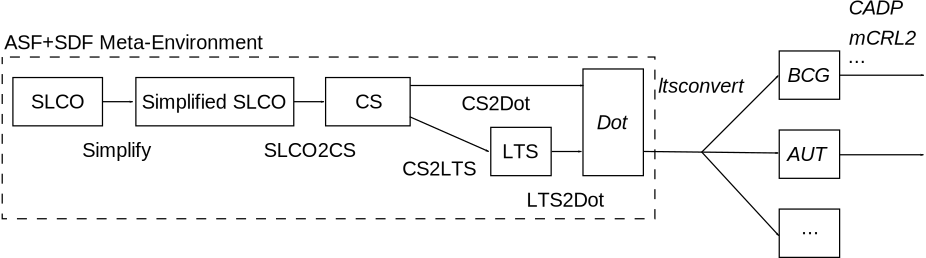
\includegraphics[scale=.5]{prototype-semantics/figs/Overview}
\caption{Overview of languages and tools}
\label{fig:prototype-semantics:languages_overview}
\end{figure}

In this chapter, we link \SLCO to \DOT, a language for the graphical representation of directed graphs~\cite{Ellson01graphviz�} that is also used by third-party tools to represent state spaces in the form of labeled transition systems.
This link is achieved via a number of transformation tools and intermediate languages, as shown in Figure~\ref{fig:prototype-semantics:languages_overview}.
In this figure, the names of existing languages and tools are displayed in an italic typeface.
The labeled arrows represent tools, and the rectangles represent languages.
Once the translation into \DOT has been achieved, several third-party toolsets supporting labeled transition systems are also within reach for manipulation, visualization, and verification of \SLCO models.
Our languages and transformation tools are defined and implemented in the \ASFSDFME~\cite{Brand:2001:ASF}.

The process of connecting \SLCO to \DOT involves two intermediate languages named~\CS and~\LTS.
The language~\LTS is a simple language for the representation of labeled transition systems\footnote{To avoid confusion, we only use the acronym~\LTS to refer to this representation language in this chapter and do not abbreviate the abstract concept of labeled transition systems itself.}.
Due to its simplicity and close resemblance to other representations of labeled transition systems, \LTS can easily be linked to existing languages and their supporting toolsets, such as those described in Sections~\ref{sec:prototype-semantics:visualization} and~\ref{sec:prototype-semantics:verification}, but also other languages that may be useful in the future.
Together, the tools that transform \SLCO models to labeled transition systems represented in \LTS form an executable prototype of the semantics of \SLCO.
This prototype enables investigating alternative design decisions regarding the semantics of the language.
By implementing an executable prototype of the semantics of \SLCO, we address research question~\RQ{3}.

\RQThree

While objects in an \SLCO model are defined separately and interact by communicating over channels, the \CS representation of such a model describes its behavior as a whole.
The objects are essentially merged into one (big) component, according to the communication as defined in the \SLCO model.
Thus, \CS forms, in a rather natural way, the missing link between the two languages \SLCO and \LTS.
Since the transformation that simplifies \SLCO models and the transformation from \CS to \LTS are straightforward, the transformation from simplified \SLCO to \CS essentially forms the core of the prototype semantics of \SLCO.
The transformation performed by \CStoDot is also straightforward and provides a convenient way to visualize \CS representations.

The remainder of this chapter is structured as follows.
In Section~\ref{sec:prototype-semantics:prototyping_semantics}, the intermediate languages and the transformation tools shown in Figure~\ref{fig:prototype-semantics:languages_overview} are introduced.
We show how third-party tools can be applied to visualize the state-spaces of \SLCO models and explain how these visualizations facilitated the development of \SLCO and its accompanying model transformations in Section~\ref{sec:prototype-semantics:visualization}.
In Section~\ref{sec:prototype-semantics:verification}, applying existing tools for verification of \SLCO models is discussed.
Section~\ref{sec:prototype-semantics:Related_Work} addresses the related work, and Section~\ref{sec:prototype-semantics:Conclusions_and_Future_Work} concludes the chapter and gives directions for future research.
